\section{ER-діаграма}

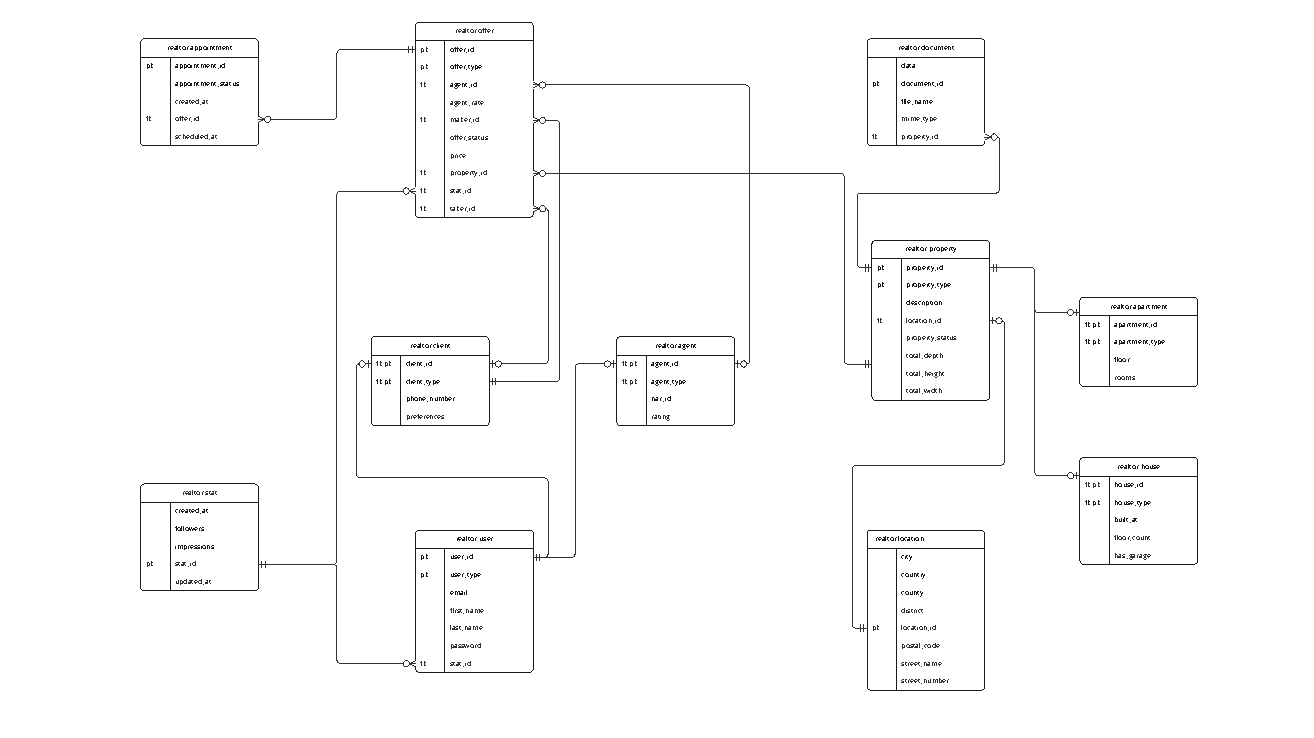
\includegraphics[width=1\linewidth]{../assets/er.pdf}

\section{Сутності}

\begin{enumerate}
    \item \textbf{location}
          Містить інформацію про географічні точки.
          \begin{enumerate}
              \item city
              \item country
              \item county
              \item district
              \item location\_id
              \item postal\_code
              \item street\_name
              \item street\_number
          \end{enumerate}

    \item \textbf{stat}
          Містить спільні для усіх сутностей статистичні або аналітичні дані.
          \begin{enumerate}
              \item created\_at
              \item followers
              \item impressions
              \item stat\_id
              \item updated\_at
          \end{enumerate}

    \item \textbf{property}
          Базовий тип для зберігання загальної інформації про всі типи об'єктів нерухомості.
          \begin{enumerate}
              \item property\_id
              \item property\_type
              \item description
              \item location\_id
              \item property\_status
              \item total\_depth
              \item total\_height
              \item total\_width
          \end{enumerate}

    \item \textbf{apartment}
          Спеціалізована таблиця для квартир
          \begin{enumerate}
              \item apartment\_id
              \item apartment\_type
              \item floor
              \item rooms
          \end{enumerate}

    \item \textbf{house}
          Спеціалізована таблиця для будинків
          \begin{enumerate}
              \item house\_id
              \item house\_type
              \item built\_at
              \item floor\_count
              \item has\_garage
          \end{enumerate}

    \item \textbf{document}
          Описує додатки, що будуть завантаженні користувачем під час створення опису об'єкта нерухомості.
          \begin{enumerate}
              \item data
              \item document\_id
              \item file\_name
              \item mime\_type
              \item property\_id
          \end{enumerate}

    \item \textbf{user}
          Базовий тип для зберігання загальної інформації про всі типи користувачів.
          \begin{enumerate}
              \item user\_id
              \item user\_type
              \item email
              \item first\_name
              \item last\_name
              \item password
              \item stat\_id
          \end{enumerate}

    \item \textbf{agent}
          Спеціалізована таблиця для агентів з нерухомості
          \begin{enumerate}
              \item agent\_id
              \item agent\_type
              \item nar\_id
              \item rating
          \end{enumerate}

    \item \textbf{client}
          Спеціалізована таблиця для клієнтів
          \begin{enumerate}
              \item client\_id
              \item client\_type
              \item phone\_number
              \item preferences
          \end{enumerate}

    \item \textbf{offer}
          Головна сутність системи. "God-object". Пов'язує агента, двох клієнтів та об'єкт нерухомості.
          \begin{enumerate}
              \item offer\_id
              \item offer\_type
              \item agent\_id
              \item agent\_rate
              \item maker\_id
              \item offer\_status
              \item price
              \item property\_id
              \item stat\_id
              \item taker\_id
          \end{enumerate}

    \item \textbf{appointment}
          Заплановані візити агентів та клієнтів до об'єктів нерухомості для огляду.
          \begin{enumerate}
              \item appointment\_id
              \item appointment\_status
              \item created\_at
              \item offer\_id
              \item scheduled\_at
          \end{enumerate}
\end{enumerate}

\section{Зв'язки}

Дизайн Class Table Inheritance є однією з імплементацій паттерну
Generalization/Specialization та використовує зв'язки 0.1-to-1
для імітації наслідування в реляційних базах даних. Його недоліком є
можливість появи осиротілих записів, що потребує додаткових перевірок
використовуючи тригери, двосторонні (deferred) зовнішні ключі,
або періодичний процес їх пошуку та видалення.

\begin{enumerate}
    \item 0.1 agent - 1 user, інакше осиротілий запис
    \item 0.1 apartment - 1 property, інакше осиротілий запис
    \item 0.M appointment - 1 offer
    \item 0.1 client - 1 user, інакше осиротілий запис
    \item 0.M document - 1 property
    \item 0.1 house - 1 property, інакше осиротілий запис
    \item 0.M offer - 0.1 agent
    \item 0.M offer - 1 client
    \item 0.M offer - 0.1 client
    \item 0.M offer - 1 property
    \item 0.M offer - 1 stat
    \item 0.1 property - 1 location
    \item 0.M user - 1 stat
\end{enumerate}
